\section*{A1\hspace{1em}Example predictions by minutely network (section~\ref{sec:aao-comparison})}

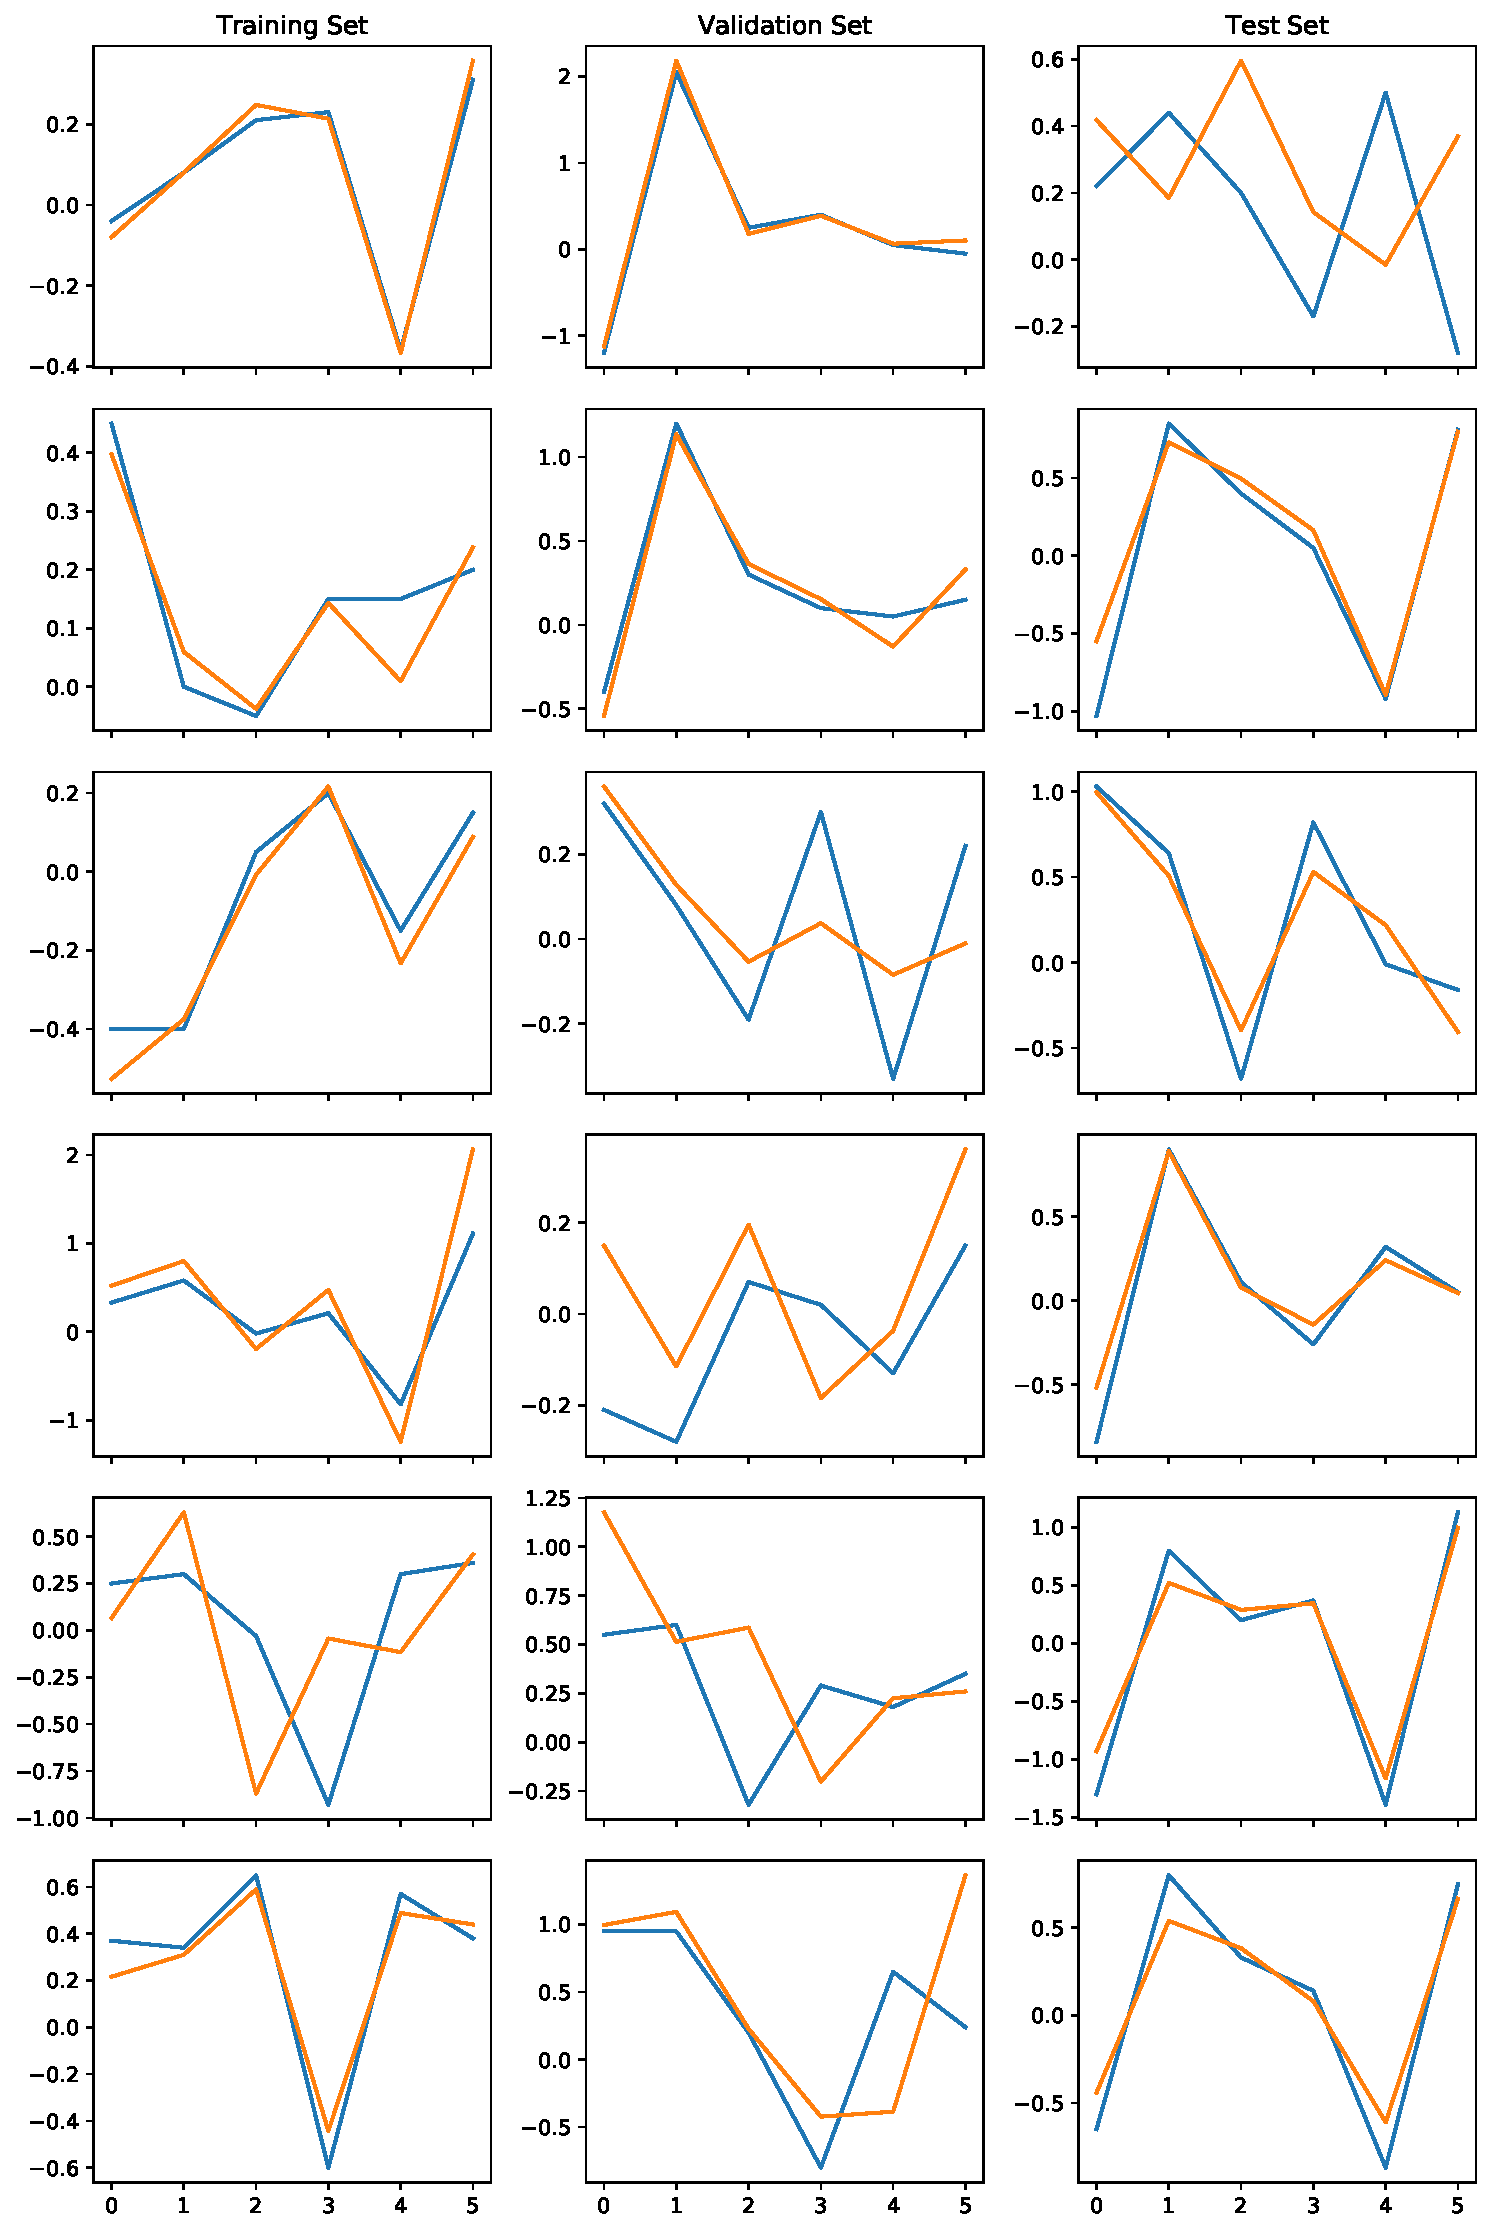
\includegraphics[width=0.95\linewidth]{minutely-prediction-samples}

\section*{A2\hspace{1em}Spread prices by leg}

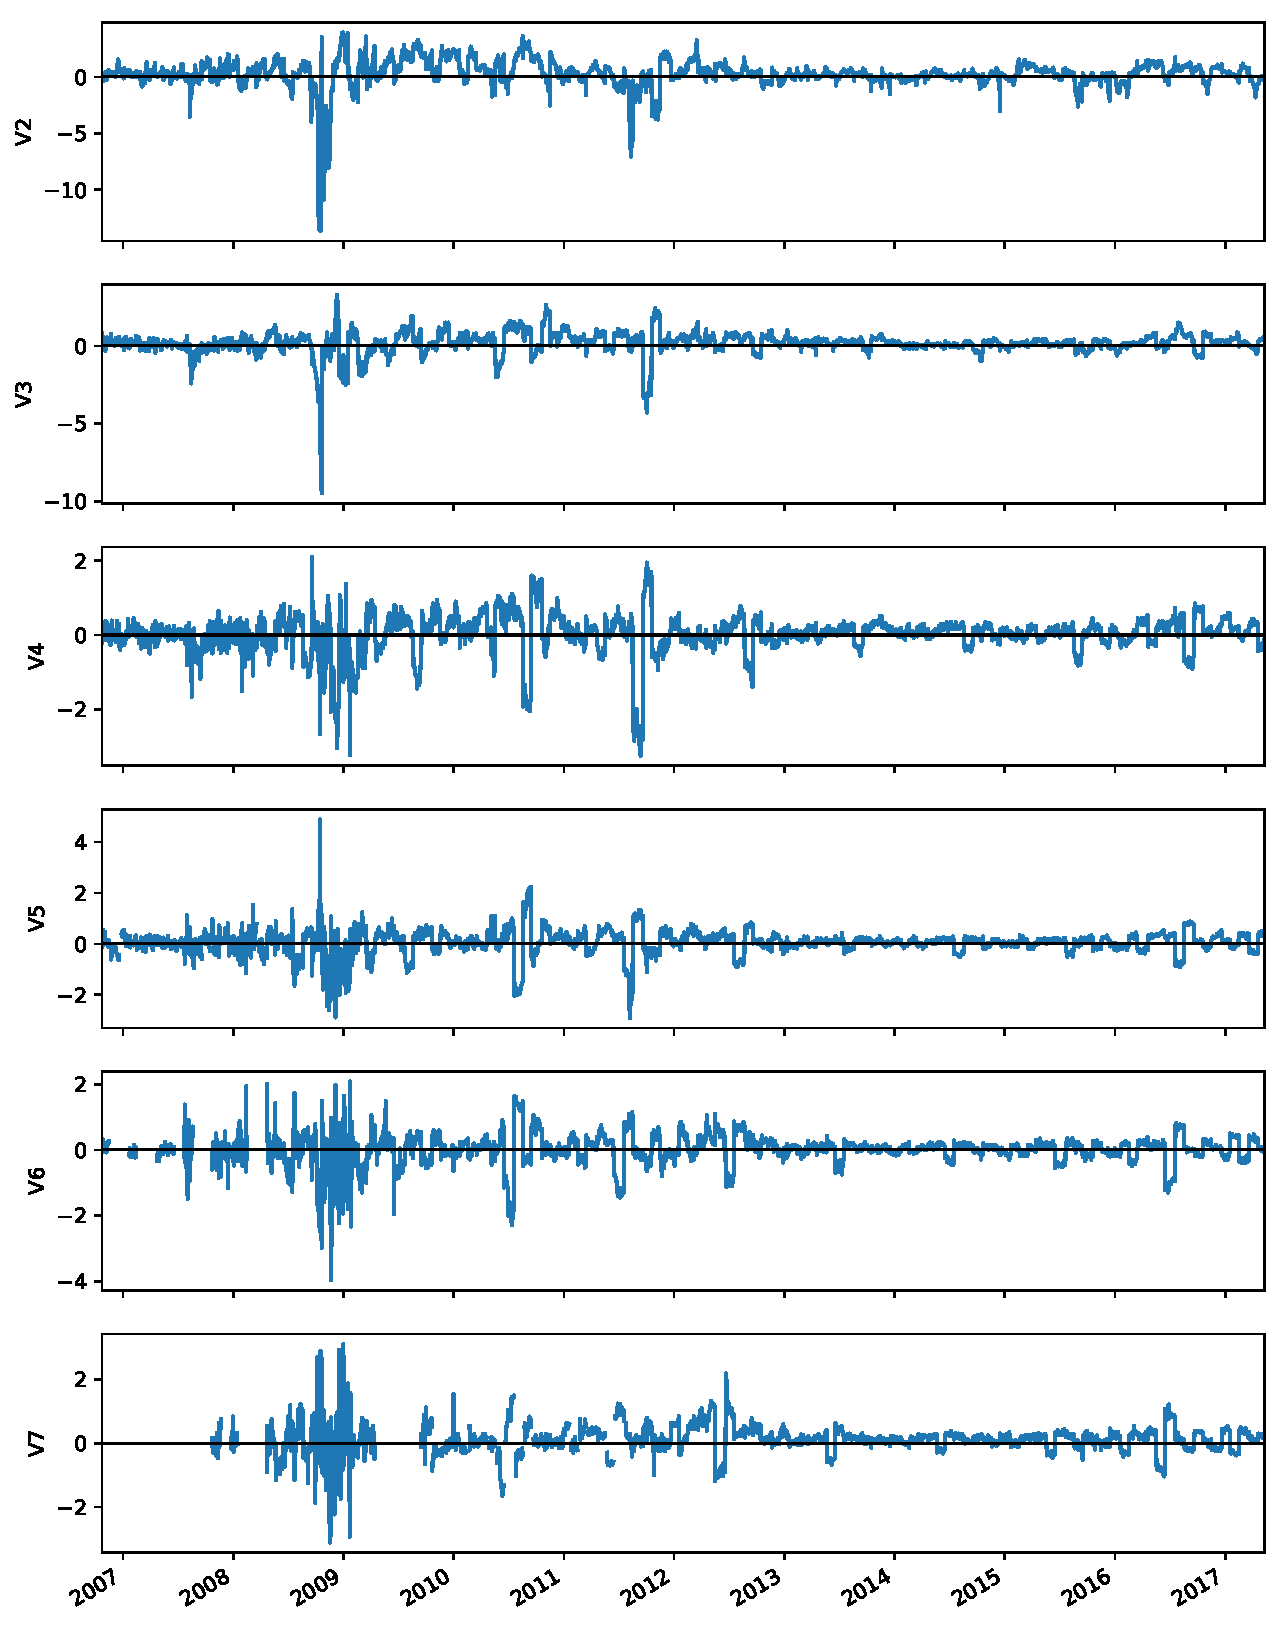
\includegraphics[width=0.99\linewidth]{spreads-legwise}

\section*{A3\hspace{1em}Spread prices by month}

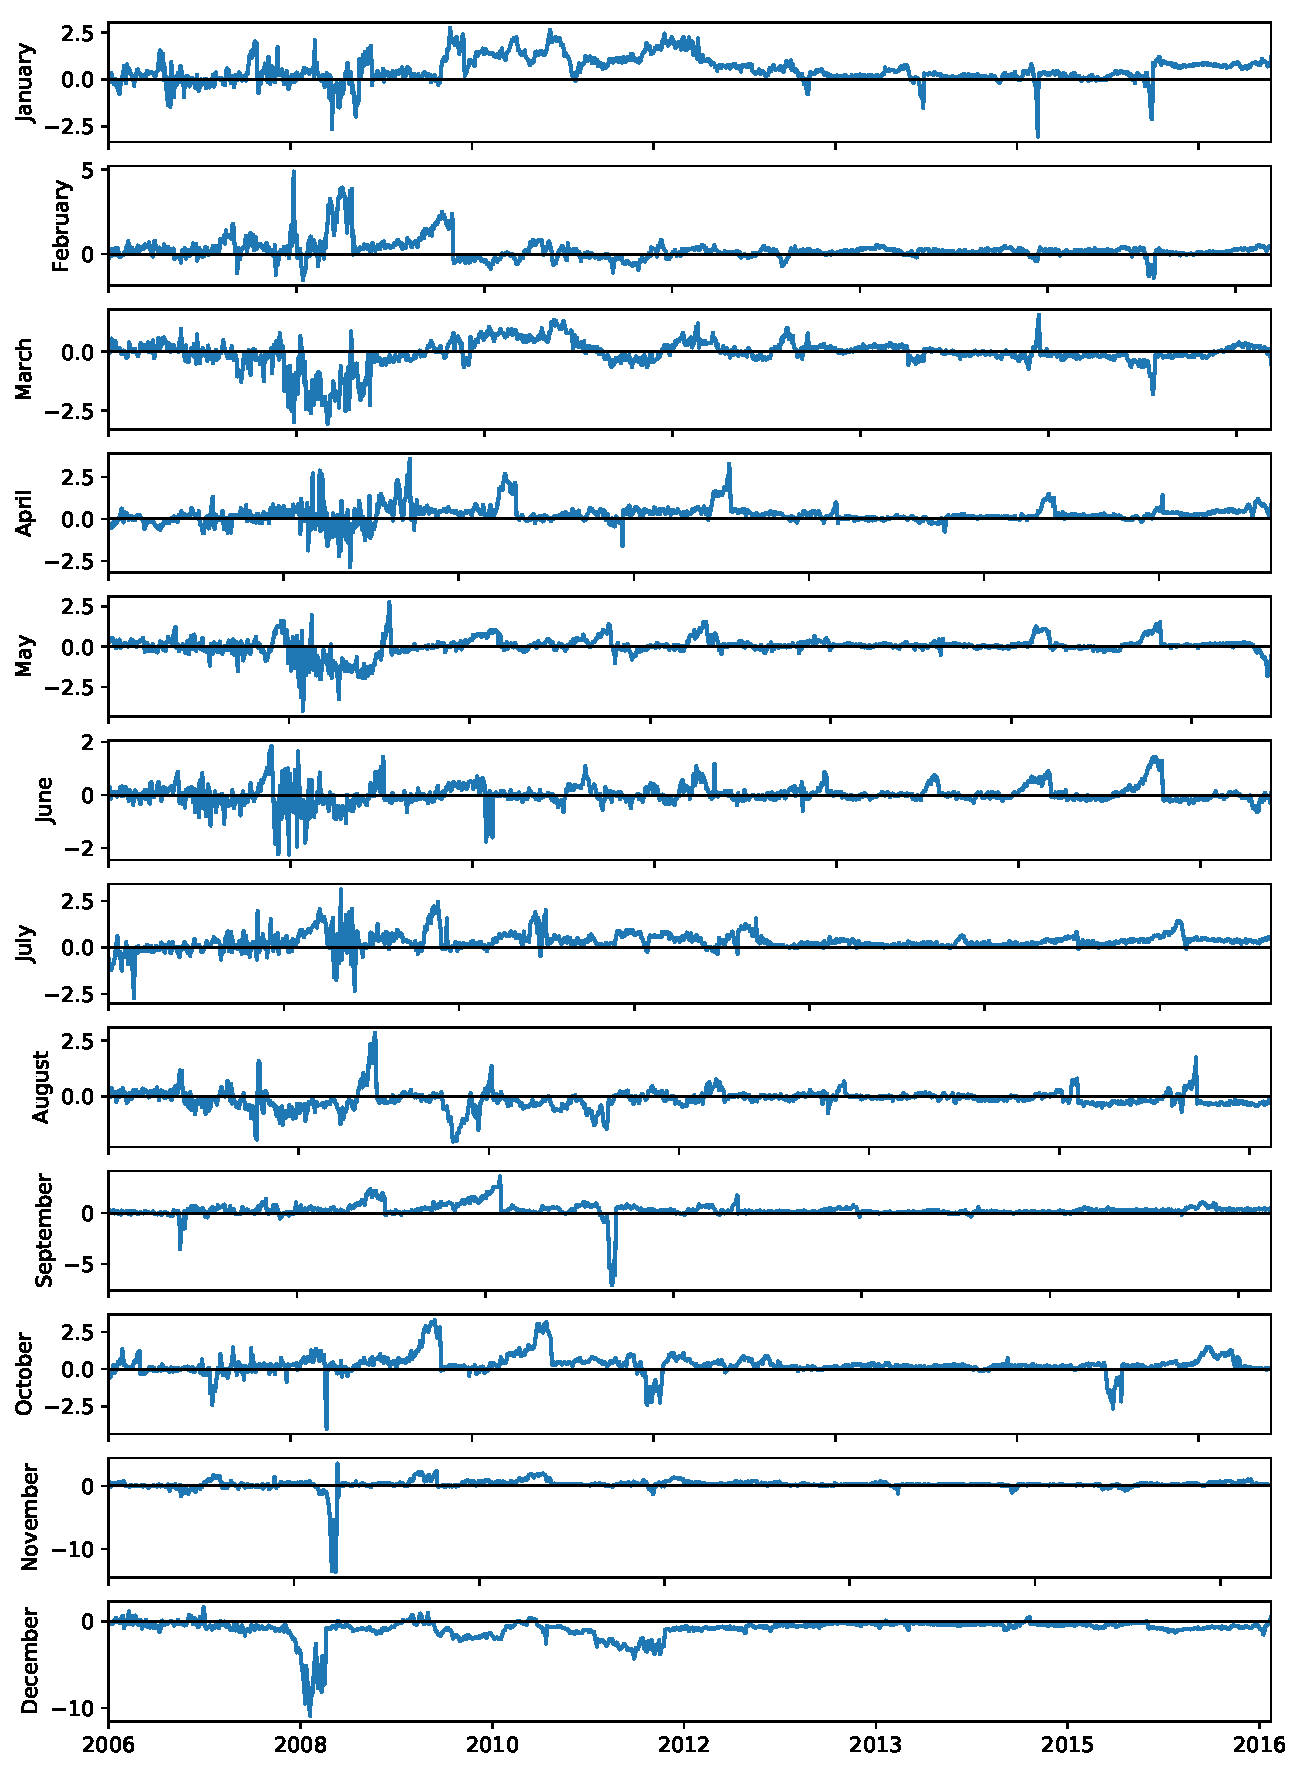
\includegraphics[width=0.99\linewidth]{spreads-monthwise}

\section*{A4\hspace{1em}Classification network's configuration}

Hyperparameters:

\begin{itemize}
	\item Number of classes $C=3$
	\item Activation functions: Mostly ReLU (same as above). At the last layer the softmax function is used: $f(z)_j = \frac{e^{z_j}}{\sum_{i=1}^C e^{z_i}}$ where $j \in \{1,\dots,C\}$
	\item Loss function: Categorical cross entropy
	\item Optimization method: Adam (same as above)
	\item Weight initializations: Using \eqref{eq:glorot-initialization} (same as above)
	\item Network depth $L = 1$
	\item Network width $K = 30$
\end{itemize}

Furthermore, during training there is scaling applied to the loss function to reflect the imbalanced ratio of samples per category. Otherwise the network would likely learn to always predict the first category as it is overrepresented in the dataset as seen below.

\vspace{1em}

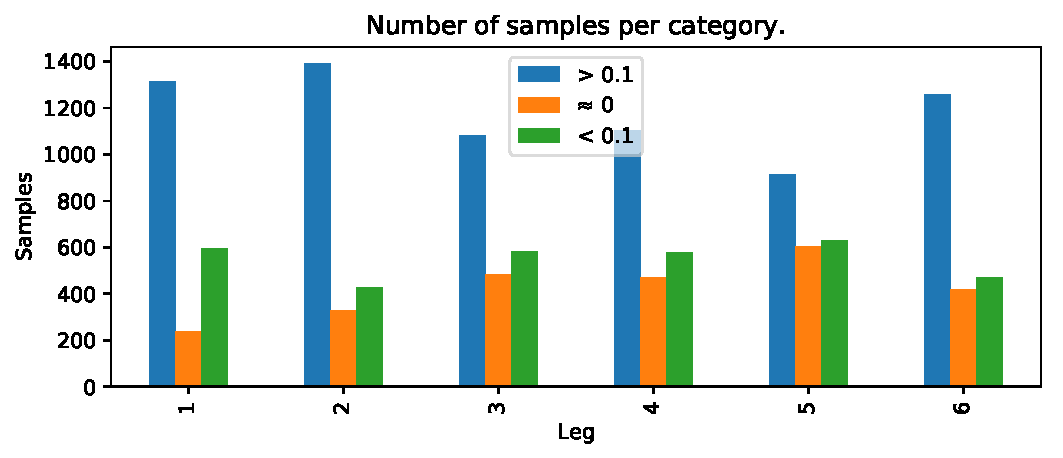
\includegraphics[width=0.9\linewidth]{classification-samples-per-category}